\chapter{Curvature}
Our intuitive notion of curvature arises mainly from two-dimensional surfaces which are embedded in ordinary three-dimensional Euclidean space. We normally think of a surface as curved because of the way it bends in R3. In chapter 9, we will capture this notion by defining the extrinsic curvature of a surface embedded in a higher dimensional space. However, our interest here is to investigate the curvature of spacetime. Our spacetime manifold M with spacetime metric gab is not naturally embedded (at least so far as we know) in a higher dimensional space. Thus we wish to develop an intrinsic notion of curvature that can be applied to any manifold without reference to a higher dimensional space in which it might be embedded.

Such a notion of curvature can be defined in terms of parallel transport. On a surface such as a plane (\figref{3.1}) or sphere (\figref{3.2}), we have an intuitive notion (which will be made mathematically precise below) of what it means to keep a vector ``pointing in the same direction'' (but always in the tangent space of the manifold) as one moves it along a path. On the plane, if one parallel-transports a vector around any closed path, the final vector always coincides with its initial value. However, this is not so on the sphere. The vector shown in Figure 3.2 comes back rotated with respect to its initial value when carried along the path shown. This basic idea allows us to characterize the plane as flat, the sphere as curved, and more generally allows us to characterize the curvature of any manifold intrinsically once we are told how to ``parallel transport'' vectors along curves. 

An alternative characterization of curvature also can be given as follows. A geodesic is a curve whose tangent is parallel-transported along itself, that is, it is a ``straightest possible'' curve. A space will be curved if and only if some initially parallel geodesics fail to remain parallel, i.e., Euclid's fifth postulate fails.

\begin{figure}[!ht]
\begin{minipage}{.48\textwidth}
    \centering
    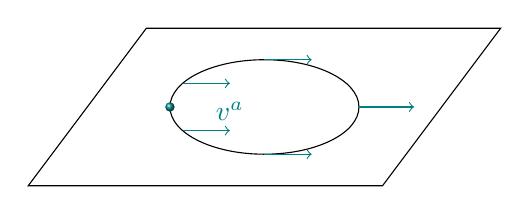
\begin{tikzpicture}
        \draw (0,0) -- (4.5,0) -- (6,2) -- (1.5,2) -- cycle;
        \draw [xshift=3cm,yshift=1cm] (0,0) ellipse (1.2 and .6);
        \draw [xshift=3cm,yshift=1cm,->,teal] (0,.6) -- (.6,.6);
        \draw [xshift=3cm,yshift=1cm,->,teal] (1.2,0) -- (1.9,0);
        \draw [xshift=3cm,yshift=1cm,->,teal] (0,-.6) -- (.6,-.6);
        \draw [xshift=3cm,yshift=1cm,->,teal] ({-1.2*cos(30)},{-.6*sin(30)}) --++ (.6,0) node [above] {$v^a$};
        \draw [xshift=3cm,yshift=1cm,->,teal] ({-1.2*cos(30)},{.6*sin(30)}) --++ (.6,0);
        \shade [xshift=3cm,yshift=1cm,ball color=teal] (-1.2,0) circle (.06);
    \end{tikzpicture}
    \caption{The parallel transport of a vector, $v^a$, around a closed curve in the plane. The vector $v^a$ always ``comes back'' pointing in the same direction as it did initially.}
    \label{3.1}
\end{minipage}
\hfill
\begin{minipage}{.48\textwidth}
    \centering
    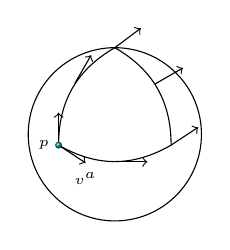
\begin{tikzpicture}[scale=.55]
        \draw (0,0) circle (2);
        \draw (0,2) edge [bend right] ({-3*sqrt(3)/4},-1/4) ({-3*sqrt(3)/4},-1/4) edge [bend right] ({3*sqrt(3)/4},-1/4) ({3*sqrt(3)/4},-1/4) edge [bend right] (0,2) -- cycle;
        \draw [->] (0,2) --++ ({.75*cos(36.8)},{.75*sin(36.8)});
        \draw [->,xshift=9*cos(30)*1pt,yshift=9*sin(30)*1pt] ({3*sqrt(3)/8},1) --++ ({.75*cos(30)},{.75*sin(30)});
        \draw [->] ({3*sqrt(3)/4},-1/4) --++ ({.75*cos(33.4)},{.75*sin(33.4)});
        \draw [->,yshift=(-1/4*1cm-11pt)] (0,0) --++ (.75,0);
        \draw [->] ({-3*sqrt(3)/4},-1/4) --++ ({.75*cos(33.4)},{-.75*sin(33.4)}) node [below] {$\scriptscriptstyle v^a$};
        \draw [->] ({-3*sqrt(3)/4},-1/4) --++ ({.75*cos(90)},{.75*sin(90)}) node [at start,left] {$\scriptscriptstyle p$};
        \draw [->,xshift=-9*cos(30)*1pt,yshift=10*sin(30)*1pt] ({-3*sqrt(3)/8},1) --++ ({.75*cos(60)},{.75*sin(60)});
        \shade [ball color=teal] ({-3*sqrt(3)/4},-1/4) circle (.08);
    \end{tikzpicture}
    \caption{The parallel transport of a vector, $v^a$, around a closed curve on the sphere. In the case shown here of a closed curved composed of three mutually orthogonal segments of great circles, the vector $v^a$ comes back rotated by $90^\circ$.}
    \label{3.2}
\end{minipage}
\end{figure}

Given only the manifold structure of space, we do not have a natural notion of parallel transport. The reason is that the tangent space $V_p$ and $V_q$, of two distinct points $p$ and $q$ are different vector spaces and hence there is no way of saying that a vector at $p$ is the same as a vector at $q$. Thus, the definition of parallel transport requires more than just the manifold structure. It is not difficult to convince oneself that a notion of how to parallel-transport vectors should be equivalent to the knowledge of how to take derivatives of vector fields. If we know how to parallel-transport vectors along a curve, we can define the derivative of a vector field in the direction of the curve; similarly, given a notion of derivative, we can define a vector to be parallel transported if its derivative along the given curve is zero. It turns out to be most convenient to work directly with the notion of a derivative operator, and we shall do so in this chapter. The failure of a vector to return to its original value when parallel transported around an infinitesimal closed curve translates into the lack of commutativity of derivatives. Thus, the notion of curvature can be defined in terms of the failure of successive differentiations on tensor fields to commute. This is the route we shall follow in section 3.2.

From where does this extra structure needed to define parallel transport or a derivative operator arise? We will show in section 3.1 that given a metric (of any signature), there is a unique definition of parallel transport which preserves inner products of all pairs of vectors. Thus, the existence of a metric gives rise to a unique notion of parallel transport and, thus, to an intrinsic notion of the curvature of the manifold. This is the notion of the curvature of a spacetime $(M,g_{ab})$ in which we are interested. However, it is more convenient to proceed by giving a general definition of the notions of derivative operator, parallel transport, and curvature before specializing to the case where they arise from a metric, and we shall proceed in this manner.

Derivative operators and parallel transport are defined in section 3.1, and curvature is defined in section 3.2. In much of our discussion in these sections, we shall follow closely the treatment given in unpublished notes of Geroch. Geodesics are introduced in section 3.3, and the geodesic deviation equation—which characterizes curvature in terms of the failure of initially parallel geodesics to remain parallel—is derived. Finally, section 3.4 discusses methods for computing curvature.

\label{3.2.3}\label{3.2.25}

\section{Derivative Operators and Parallel Transport}
A \emph{derivative operator}, $\nabla$ (sometimes called a \emph{covariant derivative}) on a manifold M is a map which takes each smooth (or merely differentiable) tensor field of type $(k,l)$ to a smooth tensor field of type $(k,l+1)$ and satisfies the five properties listed below. In the index notation, if ${T^{a_1\cdots a_k}}_{b_1\cdots b_l}\in\mathscr{T}(k,l)$, we denote the tensor field resulting from the action of $\nabla$ on $T$ by $\nabla_c{T^{a_1\cdots a_k}}_{b_1\cdots b_l}.$ It is often notationally A
convenient to attach an index directly to the derivative operator and write it as $\nabla_a$, although this is to some extent an abuse of the index notation since $\nabla_a$ is not a dual vector. Expressed in the index notation, the five conditions required of a derivative operator are

\begin{enumerate}
    \item Linearity: For all $A, B\in \mathscr{T} (k,l) $ and $\alpha, \beta\in R$
    \[\nabla_c(\alpha{A^{a_1\cdots a_k}}_{b_1\cdots b_l}+\beta {B^{a_1\cdots a_k}}_{b_1\cdots b_l})=\alpha\nabla_c{A^{a_1\cdots a_k}}_{b_1\cdots b_l}+\beta\nabla_c{B^{a_1\cdots a_k}}_{b_1\cdots b_l}\]
    \item Leibnitz rule: For all $A\in\mathscr{T}(k,l),B\in\mathscr{T}(k',l')$
    \[\nabla_e[{A^{a_l\cdots a_k}}_{b_l\cdots b_l}{B^{c_l\cdots c_k'}}_{d_1\cdots d_l'}]=[\nabla_e{A^{a_l\cdots a_k}}_{b_l\cdots b_l}]{B^{c_l\cdots c_k}}_{d_1\cdots d_l'}+{A^{a_l\cdots a_k}}_{b_1\cdots b_l}[\nabla_e{B^{c_l\cdots c_k'}}_{d_1\cdots d_l'}]\]
    \item Commutativity with contraction: For all $A\in\mathscr{T}(k,l)$
    \[\nabla_{d}({A^{a_1\cdots c\cdots a_k}}_{b_1\cdots c\cdots b_l})={\nabla_{d}A^{a_1\cdots c\cdots a_k}}_{b_1\cdots c\cdots b_l}\]
    \item Consistency with the notion of tangent vectors as directional derivatives on scalar fields: For all $f\in\mathscr{F}$ and all $t^a\in V_p$
    \[t(f)=t^a\nabla_af\]
    \item Torsion free\footnote{If condition 5 is not imposed, it can be shown that there must exist a tensor ${T^c}_{ab}$ antisymmetric in $a$ and $b$ such that $\nabla_a\nabla_bf-\nabla_b\nabla_af=-{T^c}_{ab}\nabla_cf($see problem l). ${T^c}_{ab}$ is called the torsion tensor, and thus our condition 5 states that the torsion tensor vanishes.}: For all $f\in\mathscr{F}$ 
    \[
    \nabla_a\nabla_bf=\nabla_b\nabla_af
    \]
\end{enumerate}

The fifth condition is sometimes dropped, and indeed there are theories of gravitation where it is not imposed. However, in general relativity the derivative operator is assumed to satisfy condition 5 and, unless otherwise stated, all derivative operators considered in this book will be assumed to be torsion free.

It is worth noting that the conditions 4 and 5 together with the Leibnitz rule allow us to derive a simple expression for the commutator of two vector fields $v^a$, $w^b$ in terms of any derivative operator $\nabla_a$. Applied to any smooth function $f$, we have

\begin{equation}
\begin{aligned}\relax
[v,w](f)&=v\{w(f)\}-w\{v(f)\}=v^a\nabla_a(w^b\nabla_bf)-w^a\nabla_a(v^b\nabla_bf)\\
&=\{\upsilon^a\nabla_aw^b-w^a\nabla_av^b\}\nabla_bf
\end{aligned}
\label{3.1.1}
\end{equation}

Thus we have
\begin{equation}
    [v,w]^b=v^a\nabla_aw^b-w^a\nabla_av^b
\end{equation}

Our first important task is to show that derivative operators exist. Let $\psi$ be a coordinate system and let $\{\partial/\partial
x^\mu\}$ and $\{\d x^\mu\} $ be the associated coordinate bases. Then n the region covered by these coordinates we may define a derivative operator, $\partial_a$, called an ordinary derivative, as follows. For any smooth tensor field $T{^{a_1\cdots a_k}}_{b_1\cdots b_k}$ we take its components $T^{\mu_1\cdots\mu_k}$ in this coordinate basis and define $\partial_c{T^{a_1\cdots a_k}}_{b_1\cdots b_l}$ to be the tensor whose components in this coordinate basis are the bartial derivatives $\partial({T^{\mu_1\cdots\mu_k}}_{\nu_1\cdots\nu_l})/\partial x^\sigma$. All five conditions follow immediately from the standard properties of partial derivatives. Indeed, by the equality of mixed partial derivatives, the fifth condition holds for all tensor fields, not just scalar fields. Thus, given a coordinate system $\psi$, we can construct an associated derivative operator $\partial_a.$ Df course, a different choice of coordinate system $\psi'$ will yield a different derivative operator $\partial_a'$, that is, the components of the tensor $\partial_c{T^{a_j\cdots a_k}}_{b_1\cdots b_l}$ in the new (primed) coordinates will $not$ be equal to the partial derivatives of the primed components of ${T^{a_1\cdots a_k}}_{b_1\cdots b_l}$ with respect to the primed coordinates. Thus, a given ordinary derivative operator is coordinate dependent, i.e., it is not naturally associated with the structure of the manifold.

How unique are derivative operators? By condition (4), any two derivative operators $\nabla_a$ and $\tilde{\nabla}_a$ must agree in their action on scalar fields. To investigate their possible disagreements on tensors of the next highest rank, let $\omega_b$ be a dual vector field and consider the difference $\tilde{\nabla}_a(f\omega_b)-\nabla_a(f\omega_b)$ for an arbitrary scalar field $f$. By the Leibnitz rule we have
\begin{equation}
    \tilde{\nabla}_a(f\omega_b)-\nabla_a(f\omega_b)=(\tilde{\nabla}_af)\omega_b+f\tilde{\nabla}_a\omega_b-(\nabla_af)\omega_b-f\nabla_a\omega_b=f(\tilde{\nabla}_a\omega_b-\nabla_a\omega_b)    
    \label{3.1.3}
\end{equation}

where we have used property (4) again. Now at a point $p,\tilde{\nabla}_a\omega_b$ and $\nabla_a\omega_b$ each depend on how $\omega_b$ changes as one moves away from $p$. However, \eqref{3.1.3} shows hat their difference $\tilde{\nabla}_a\omega_b-\nabla_a\omega_b$ depends only on the value of $\omega_b$ at point $p$. To see his, we suppose that $\omega_b'$ equals $\omega_b$ at $p$ and show that we get the same answer if we replace $\omega_b$ by $\omega_b'$. By problem 2 of chapter 2, it follows that since $\omega_b'-\omega_b$ vanishes at $p$ we can find smooth functions, $f_{(a)}$, which vanish at $p$ and smooth dual vector fields, $\mu_b^{(\alpha)}$, such that

\begin{equation}
    \omega_b'-\omega_b=\sum_{\alpha=1}^{n}f_{(\alpha)}\mu_b^{(\alpha)}
    \label{3.1.4}
\end{equation}

Hence, using \eqref{3.1.3}, at point $p$ we have
\begin{equation}
\begin{aligned}
    \tilde{\nabla}_a(\omega_b'-\omega_b)-\nabla_a(\omega_b'-\omega_b)&=\sum_{\alpha}\ab\{\tilde{\nabla}_a\ab(f_{(\alpha)}\mu_b^{(\alpha)})-\nabla_a\ab(f_{(\alpha)}\mu_b^{(\alpha)})\}\\
    &=\sum_{\alpha}f_{(\alpha)}\ab\{\tilde{\nabla}_a\mu_b^{(\alpha)}-\nabla_a\mu_b^{(\alpha)}\}=0
\end{aligned}
\label{3.1.5}
\end{equation}

since each $f_{(\alpha)}=0$ at $p$. Thus, we have
\begin{equation}
    \tilde{\nabla}_a\omega_b'-\nabla_a\omega_b'=\tilde{\nabla}_a\omega_b-\nabla_a\omega_b
    \label{3.1.6}
\end{equation}

which proves our assertion.

Thus, we have shown that $\tilde{\nabla}_a-\nabla_a$ defines a map of dual vectors at $p$ (as opposed to dual vector fields defined in a neighborhood of $p)$ to tensors of type $(0,2)$ at $p$ By property (1), this map is linear. Consequently $(\tilde{\nabla}_a-\nabla_a)$ defines a tensor of type $(1,2)$ at $p$, which we will denote as ${C^c}_{ab}.$ Thus, we have shown that given any two derivative operators $\tilde{\nabla}_a$ and $\nabla_a$ there exists a tensor field ${C^c}_{ab}$ such that
\begin{equation}
    \nabla_a\omega_{b}=\tilde{\nabla}_a\omega_{b}-{C^c}_{ab}\omega_c
    \label{3.1.7}
\end{equation}

This displays the possible disagreements of the actions of $\nabla_a$ and $\tilde{\nabla}_a$ on dual vecton fields.

A symmetry property of ${C^c}_{ab}$ follows immediately from condition (5). If we let $\omega_{b}=\nabla_{b}f=\tilde{\nabla}_{b}f$, we find
\begin{equation}
    \nabla_a\nabla_{b}f=\tilde{\nabla}_a\tilde{\nabla}_{b}f-{C^c}_{ab}\nabla_cf
    \label{3.1.8}
\end{equation}

Since both $\nabla_a\nabla_bf$ and $\tilde{\nabla}_a\tilde{\nabla}_bf$ are symmetric in $a$ and $b$, it follows that ${C^c}_{ab}$ must also have this property
\begin{equation}
    {C^c}_{ab}={C^c}_{ba}
    \label{3.1.9}
\end{equation}

\eqref{3.1.9}, of course, need not hold if the torsion-free requirement is dropped.

The difference in the action of $\tilde{\nabla}_a$ and $\nabla_a$ on vector fields and all higher rank tenson fields is determined by \eqref{3.1.7}, the Leibnitz rule, and property (4). For every vector field $t^a$ and one-form field $\omega_a$, property (4) tells us that
\begin{equation}
    (\tilde{\nabla}_a-\nabla_a)(\omega_bt^b)=0
    \label{3.1.10}
\end{equation}

On the other hand, by the Leibnitz rule, we have
\begin{equation}
    (\tilde{\nabla}_a-\nabla_a)(\omega_bt^b)=({C^c}_{ab}\omega_c)t^b+\omega_b(\tilde{\nabla}_a-\nabla_a)t^b
    \label{3.1.11}
\end{equation}

Thus, index substituting on contracted indices, we find
\begin{equation}
    \omega_{b}\ab[(\tilde{\nabla}_a-\nabla_a)t^{b}+{C^{b}}_{ac}t^c]=0
    \label{3.1.12}
\end{equation}

for all $\omega_b$. This implies
\begin{equation}
    \nabla_at^{b}=\tilde{\nabla}_at^b+{C^{b}}_{ac}t^c
    \label{3.1.13}
\end{equation}

Continuing in a similar manner, we can derive the general formula for the action of $\nabla_a$ on an arbitrary tensor field in terms of $\tilde{\nabla} _a$ and $\tilde{c} _{ab}^c$. For $T\in\mathscr{T}(k,l)$ we find
\begin{equation}
    \nabla_a{T^{b_1\cdots b_k}}_{c_1\cdots c_l}=\tilde{\nabla}_a{T^{b_1\cdots b_k}}_{c_1\cdots c_l}+\sum_iC^{b_1}{}_{ad}T^{b_1\cdots d\cdots b_k}{}_{c_1\cdots c_l}-\sum_jC^d{}_{ac_j}T^{b_1\cdots b_l}{}_{c_1\cdots d\cdots c_l}
    \label{3.1.14}
\end{equation}

Thus, the difference between the two derivative operators $\nabla_a$ and $\tilde{\nabla}_a$ is completely characterized by the tensor field ${C^c}_{ab}.$ Conversely, it is not difficult to check that if $\tilde{\nabla}_a$ is a derivative operator and ${C^c}_{ab}$ is an arbitrary smooth tensor field which is symmetric in its lower indices, then $\nabla_{a}$ defined by equation (3.1.14) will also be a derivative operator. This shows that there is a great deal of freedom involved in the choice of a derivative operator, as on an $n$-dimensional manifold ${C^c}_{ab}$ has $n^2(n+1)/2$ independent components to be specified at each point.

The most important application of equation (3.Î.14) arises from the case where $\tilde{\nabla}_{a}$
is an ordinary derivative operator $\partial_{a}$. In this case, the tensor field ${C^c}_{ab}$ is denoted $\Gamma_{ab}^{c}$ and called a $Christoffel$ symbol. Thus, for example, we write

$$
\nabla_{a}t^{b}\:=\:\partial_{a}t^{b}\:+\:\Gamma_{\:ac}^{b}t^{c}
$$
(3.1.15) Since we know how to compute the ordinary derivative associated with a given coordinate system, equation $(\dot{3}.1.15)$ (and, more generally, eq.[3.1.14]with $\partial_{a}$ and $\Gamma_{ac}^b$ replacing $\tilde{\nabla}_a$ and $\bar{C}_{ac}^b)$ tells us how to compute the derivative $\nabla_a$ if we know $\Gamma_{ac}^b$ Note that, as defined here, a Christoffel symbol is a tensor field associated with the derivative operator $\nabla_a$ and the coordinate system used to define $\partial_a$. However, if we change coordinates, we also change our ordinary derivative operator from $\partial_a^{\prime}$ to $\partial_a^{\prime}$ and thus we change our tensor $\Gamma_{ab}^\mathrm{\vdots c}$ to a new tensor $\Gamma_{ab}^{\prime c}$. Hence the coordinate components of $\Gamma_{ab}^c$ in the unprimed coordinates will not be related to the components of $\Gamma_{ab}^{\ddots}$ in the primed coordinates by the tensor transformation law, equation (2.3.8), since we change tensors as well as coordinates.

Given a derivative operator $\nabla_{a}$ we can define the notion of the parallel transport of a vector along a curve $C$ with a tangent $t^a$. A vector $v^a$ given at each point on the curve is said to be parallelly transported as one moves along the curve if the equation
(3.1.16) $t^{a}\nabla_{a}v^{b}=0$
is satisfied along the curve. More generally, one can define the parallel transport of a tensor of arbitrary rank by

(3.1.17) 
$$
t^{a}\nabla_{a}T^{b_{1}\cdots b_{k}}_{c_{1}\cdots c_{l}}=0\quad.
$$

Choosing a coordinate system and using equation (3.1.15), we can express equation (3.1.16) as

(3.1.18) 
$$
t^{a}\partial_{a}v^{b}+t^{a}{\Gamma^{b}}_{ac}v^{c}=0\quad,
$$

or, in terms of components in the coordinate basis and the parameter $t$ along the curve,

(3.1.19) 
This shows that the parallel transport of $\upsilon^{a}$ depends only on the values of $v^a$ on the curve, so we may consider the parallel transport properties of vectors defined only along the curve as opposed to vector fields. Furthermore, from the properties of ordinary differential equations it follows that equation (3.1.19) always has a unique solution for any given initial value of $v^a$. Thus, a vector at a point $p$ on the curve uniquely defines a “parallel transported vector" everywhere else on the curve. We may use this notion of parallel transport to identify (i.e., map into each other) the tangent spaces $V_p$ and $V_q$ of points $p$ and $q$ if we are given a derivative operator and a curve connecting $p$ and $q$. The mathematical structure arising from such a curve-

\section{Curvature}
% \begin{equation}
% \nabla_a\nabla_b\omega_c-\nabla_b\nabla_a\omega_c=R_{abc}^d\omega_d
%     \label{3.2.3}
% \end{equation}

% \begin{equation}
% R_{ac}=R_{abc}^b
%     \label{3.2.25}
% \end{equation}

\section{Geodesics}
\section{Methods for Computing Curvature}

% \includepdf[pages=17-30]{document}